\chapter*{3. El mercado internacional del grano de café}

El café forma parte del conjunto de bienes agrícolas o \textit{soft commodities}, una categoría que incluye productos como el arroz, el maíz y la soya, los que comparten un conjunto de características que definen su comportamiento en los mercados globales.

Primero, se trata de productos con relativa sustituibilidad, dado que cada uno cumple funciones específicas en la dieta y el consumo, tanto a nivel individual como industria \citep{gouel2018nutrition}. Segundo, estos productos presentan una alta volatilidad de precios, la que se manifiesta en fluctuaciones de corto plazo, a pesar de presentar ciclos de precios en el mediano y largo plazo \citep{deaton1992behaviour, maurice2011unraveling, covindassamy2017sugar}. Tercero, los bienes agrícolas cuentan con largos ciclos de producción, lo que dificulta una rápida respuesta ante los cambios del mercado \citep{mehta2008responding}. Esto se suma, además, a una alta susceptibilidad a choques climáticos, como sequías, heladas o precipitaciones inusuales \citep{oic2013cincuenta}. En conjunto, todas estas características hacen que el mercado del café, al igual que el de otros \textit{soft commodities}, esté sujeto a dinámicas complejas de ajuste y riesgo, la que se puede ver afectada por el avance del cambio climático.

Lo anterior tiene dos implicancias sumamente relevantes para esta investigación. Por un lado, reafirma la relevancia de estimar el impacto del cambio climático sobre la comercialización del café, por ser un factor que afecta directamente a la producción de este bien. Por otro lado, dado que el café comparte características con otros \textit{soft commodities}, el modelo de estimación utilizado puede servir como guía para el análisis de otros bienes agrícolas.

En las últimas décadas, el comercio internacional del grano verde de café ha experimentado un crecimiento sostenido. Entre 1990 y 2019, las exportaciones globales de este grano aumentaron en un 59\%, pasando de 73.2 millones a 116.3 millones de sacos de 60 kilogramos. En este mismo período, el precio internacional del café en bolsa del bien ha aumentado en un 41\%, desde 71.5 hasta los 100.5 centavos de dólar por libra. Estas cifras son reflejo de la expansión de la demanda global y de la materialización de ciertas restricciones estructurales que presionan los precios al alza.

\begin{figure}[htbp]
    \centering
    \begin{minipage}[t]{0.45\textwidth}
        \centering
        \caption{Exportaciones mundiales de café}
        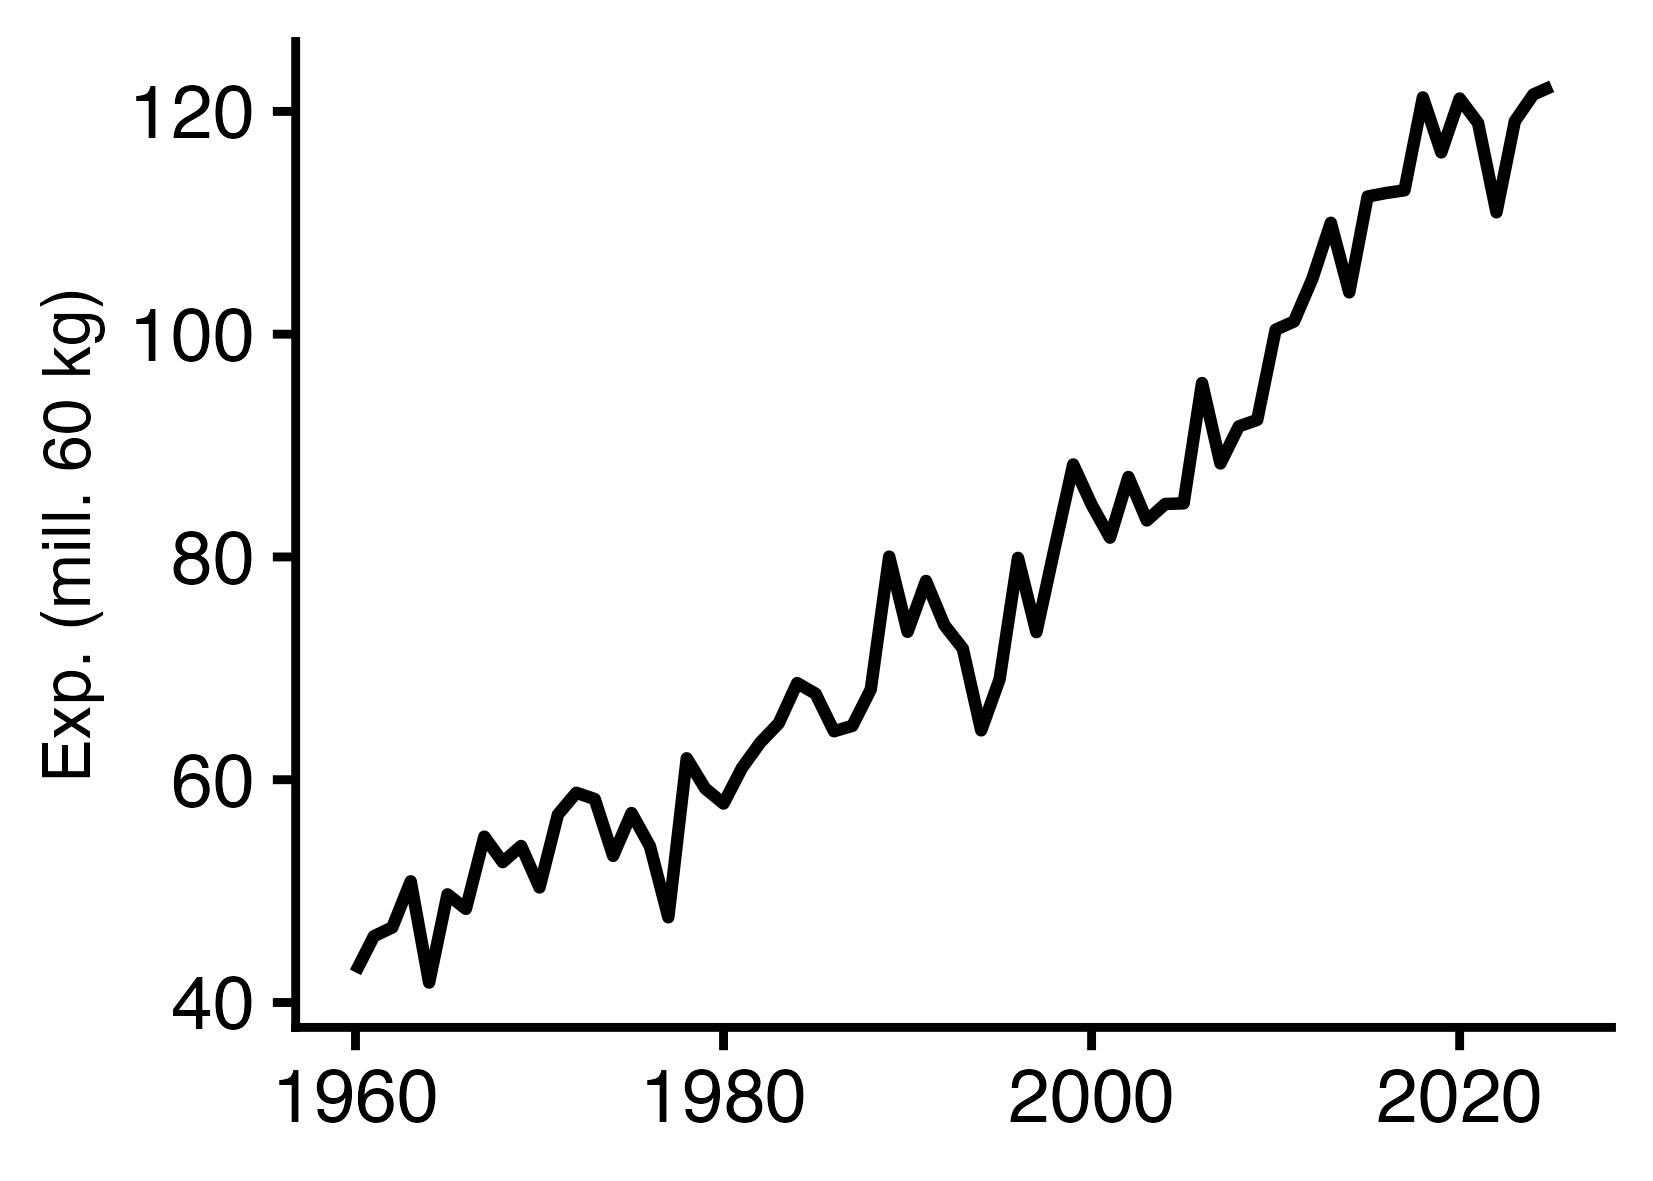
\includegraphics[width=\linewidth]{figures/export1960.png}
        \label{fig:plot03_01}
    \end{minipage}
    \hfill
    \begin{minipage}[t]{0.45\textwidth}
        \centering
        \caption{Precio internacional del café}
        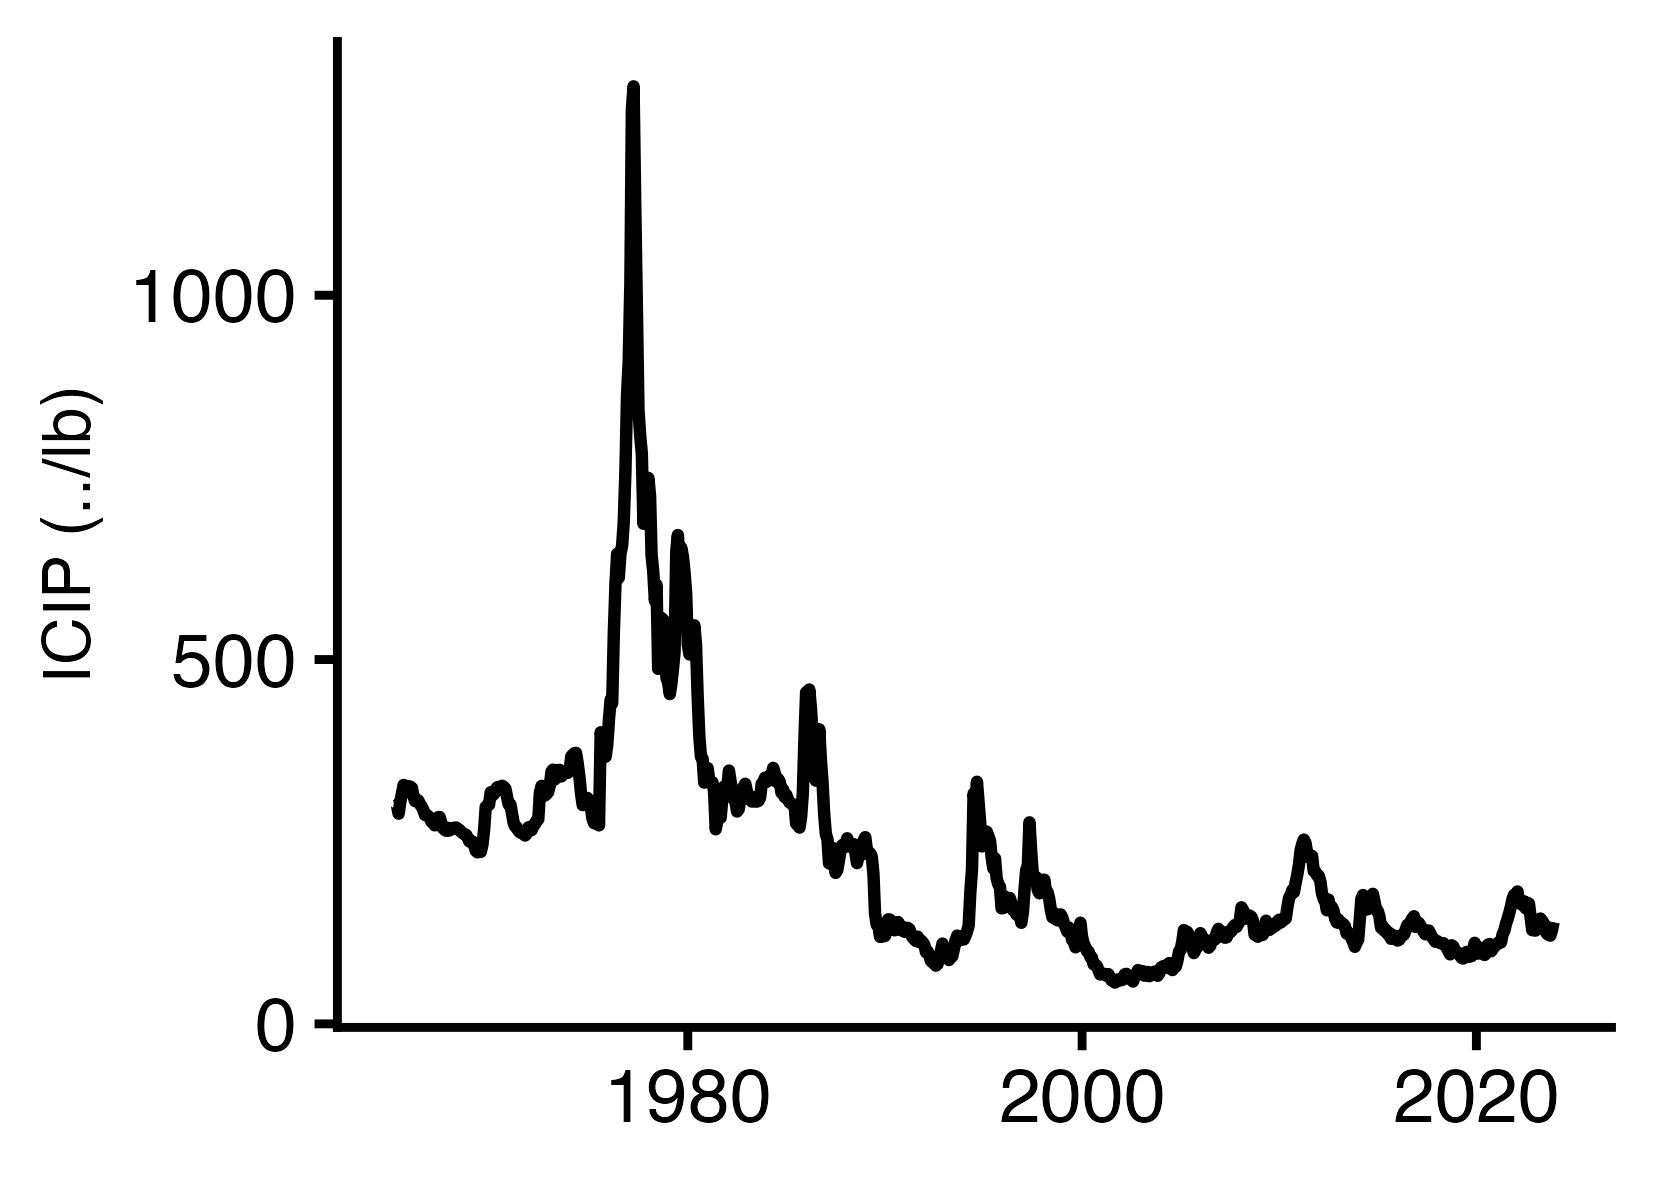
\includegraphics[width=\linewidth]{figures/icip1960.png}
        \label{fig:plot03_02}
    \end{minipage}
\end{figure}

A pesar de esta dinámica, la estructura del mercado se ha mantenido relativamente estable. Brasil ha dominado las exportaciones de las últimas tres décadas, con una participación anual promedio del 26\%, seguido por Colombia (13\%) y Viet Nam (8\%). En tanto, la UE concentra el 50\% de las importaciones, seguido por Estados Unidos (27\%) y Japón (8\%).

En resumen, se configura un patrón estructural en la economía del café. En palabras de Igami (2015): \textit{el mercado internacional del café está formado por los países desarrollados (como importadores) y los países en desarrollo (como exportadores)}. Esto se observa, por ejemplo, al comparar el Producto Interno Bruto (PIB) de cada grupo y su evolución en el tiempo. De forma consistente, los países importadores presentan un PIB mayor.

\begin{figure}[H]
    \centering
    \caption{Producto Interno Bruto para exportadores e importadores de café}
    
\includegraphics[scale = 0.9]{figures/plot3.png}
    \label{fig:plot03_03}
\end{figure}

Pero no solo existe una diferencia a nivel de ingresos, sino también con relación a la vulnerabilidad frente al cambio climático y sus consecuencias. El Índice de la Iniciativa Global de Adaptación de la Universidad de Notre Dame (ND-GAIN, por sus siglas en inglés) pondera cerca de 40 factores económicos, políticos, ambientales y sociales, a fin de estimar el grado de preparación de un país frente al cambio climático \citep{gain2024}. Nuevamente, la diferencia es relevante entre grupos. Siguiendo la interpretación del índice, los países importadores estarían mejor preparados frente a las consecuencias negativas del cambio climático -aunque con mayor varianza. Esto reafirma la apreciación de Igami y refuerza la importancia de cuantificar el impacto climático sobre el mercado internacional del café y su distribución entre grupos de países.

\begin{figure}[H]
    \centering
    \caption{Índice ND-GAIN para exportadores e importadores de café}
    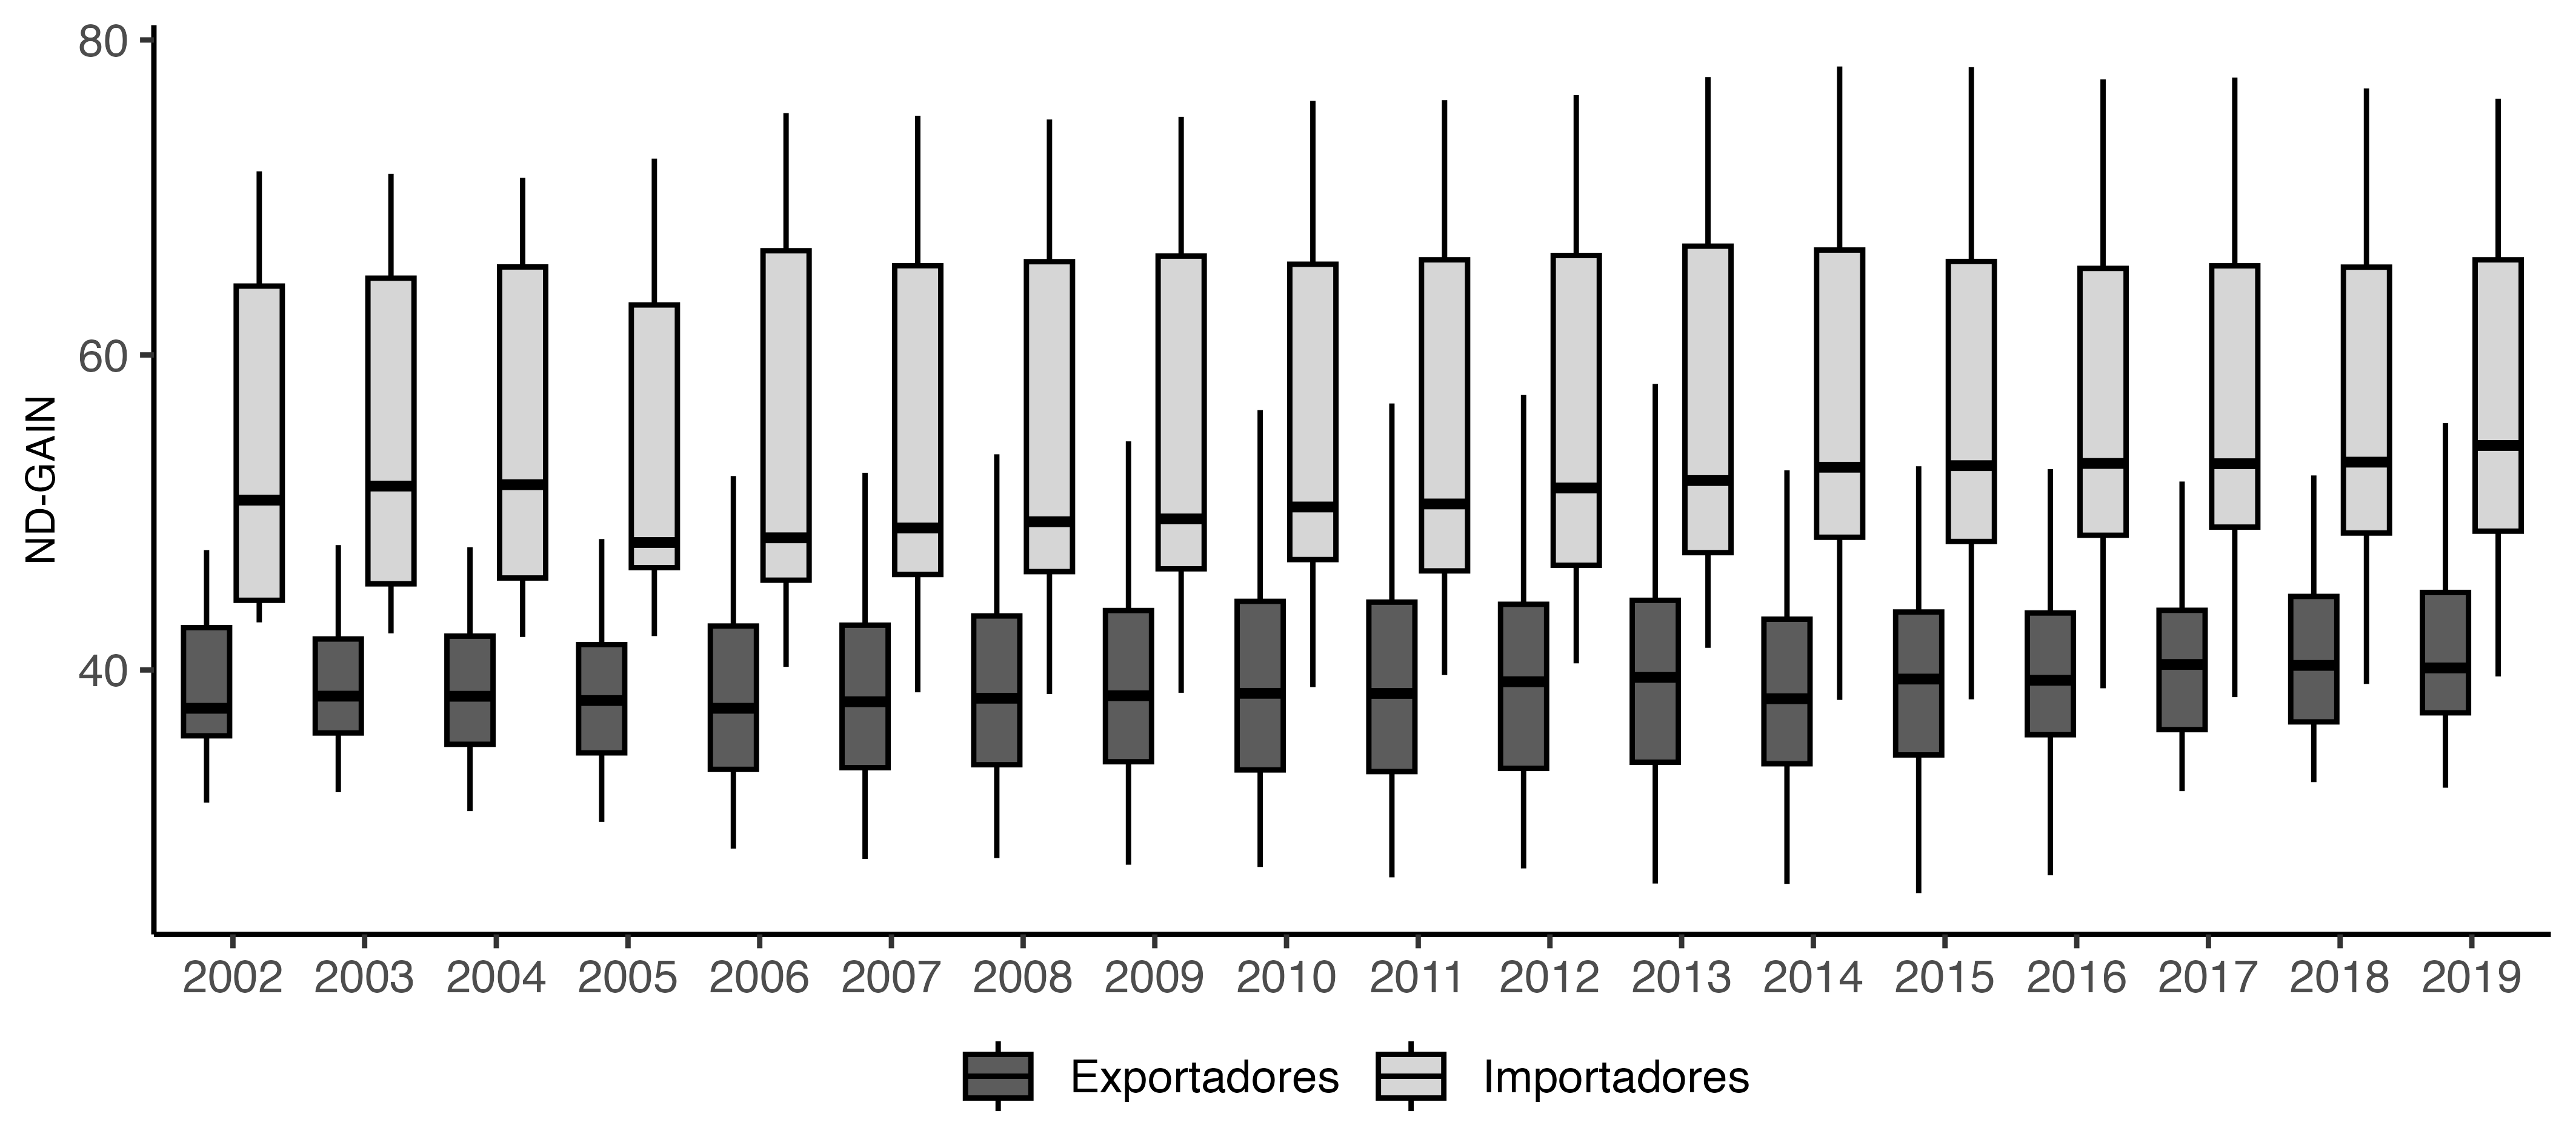
\includegraphics[scale = 0.9]{figures/plot03_09.png}
    \label{fig:plot03_09}
\end{figure}

En el plano institucional, el mercado internacional del café está representado por la Organización Internacional del Café (ICO, por sus siglas en inglés), un organismo intergubernamental que reúne a países exportadores e importadores desde su fundación en 1963. Esta organización representa a aproximadamente el 97\% de la producción mundial y el 80\% del consumo global, constituyéndose como el principal foro de coordinación y diálogo entre los actores estatales vinculados al comercio del café.

La ICO cumple funciones de monitoreo y articulación de intereses comerciales, y ha asumido un rol cada vez más activo frente a los desafíos ambientales que amenazan la sostenibilidad del sector. En respuesta al creciente impacto de fenómenos climáticos como sequías, lluvias intensas y variaciones de temperatura, la ICO ha intensificado su ejercicio de investigación y divulgación \citep{oic2013cincuenta}. Así, los informes mensuales de actualización sobre el estado del mercado suelen incluir análisis sobre el efecto más reciente del cambio climático en los países productores [CITAR]. Al mismo tiempo, los reportes anuales y quinquenales ofrecen una mirada de mediano y largo plazo sobre la relación entre cambio climático, producción y precios internacionales [CITAR].

Sumado a lo anterior, la ICO promueve activamente la investigación sobre el mercado del café, desde diferentes disciplinas, a fin de generar evidencia para el diseño de políticas y estrategias sectoriales que permitan mitigar los riesgos asociados al cambio climático y aumentar la resiliencia de los productores, garantizando la estabilidad del mercado en el futuro \citep{oic1998enso, ICO2024}.

\section*{3.1. Variedades y cadena de producción del café}

Existen dos principales variedades botánicas del grano verde de café: \textit{Coffea Arabica} (Arabica) y \textit{Coffea Canephora} (Robusta). Ambas especies dominan ampliamente el mercado mundial, representando en conjunto cerca del 99\% de la producción mundial \citep{ICO2009ClimateCoffee}.

La especie Arabica es originaria de los bosques tropicales del este de África, en zonas montañosas situadas entre los 1.500 y 2.800 metros de altitud, dentro de una franja geográfica que va desde los 4° hasta los 9° de latitud norte. En estas regiones el clima se caracteriza por una temperatura media anual entre 18°C y 22°C, con pronunciadas variaciones estacionales y una precipitación anual que oscila entre 1.600 y más de 2.000 mm, acompañada de una estación seca que suele durar entre 3 y 4 meses.

Las condiciones ideales para el cultivo y desarrollo del café Arabica se encuentran en zonas de altas montañas tropicales, como el sureste de Brasil, donde la temperatura óptima se encuentra entre los 18°C y 23°C. Sobre este rango, el desarrollo y la maduración de los frutos tiende a acelerarse, lo que habitualmente reduce la calidad del grano. Además, una exposición prolongada a temperaturas diarias por sobre los 30°C puede afectar negativamente el crecimiento de las plantas y generar anomalías en ellas.

Por su parte, el café de especie Robusta tiene su origen en los bajos bosques de África central, específicamente en la cuenca del río Congo, extendiéndose hasta regiones cercanas al lago Victoria y Uganda. A diferencia de la especie Arabica, la familia Robusta prospera en climas cálidos y húmedos, con temperaturas medias anuales entre 23°C y 26°C, una baja variabilidad térmica estacional y una precipitación abundante (superior a los 2.000 mm anuales) que se distribuye a lo largo de 9 a 10 meses en el año. Sin embargo, temperaturas muy altas, en especial si van acompañadas de un aire seco, pueden resultar perjudiciales. Asimismo, esta especie no resiste temperaturas inferiores a 6°C ni exposiciones prolongadas a valores cercanos a los 15°C.

El modelo utilizado en esta investigación, y que será explicado en detalle en la sección 5, considera la transacción de un sólo bien homogéneo, sin perjuicio de las variedades previamente señaladas. Esta aproximación surge de la manera en que la industria ha sido gestionada históricamente y de la modelación típica en la literatura académica. Sin embargo, la incorporación de las diferencias entre las variedades de cada grano de café permitiría una mejor identificación del impacto del estrés térmico, pues agregaría mayor precisión al distinguir entre las condiciones ambientales que favorecen el desarrollo de cada cultivo.

Una de las principales razones para esta consideración radica en la gestión y operación de organismos internacionales, y otros acuerdos históricos. La ICO, por ejemplo, calcula un índice global de precios del café que pondera la relevancia de cada especie para generar un precio agregado que afecta a todo el mercado, con independencia del tipo de grano comercializado. También se debe tener presente que el Acuerdo Internacional del Café (ICA), que consistía en la repartición de cuotas de exportación entre los países de la ICO y que estuvo vigente entre 1965 y 1989, funcionaba en base a este índice agregado, lo que se traduce en un entendimiento del café como un bien homogéneo.

Adicionalmente, la literatura académica ha caracterizado los granos de café como bienes homogéneos a fin de ser coherente con su dinámica y con el funcionamiento del cartel recién mencionado. Este supuesto simplifica el análisis económico y facilita la medición del poder de mercado entre países. Al modelar el café como un producto homogéneo, los investigadores pueden centrarse en aspectos macro como las elasticidades de la oferta y la demanda, o los efectos de los choques externos en el precio y el volumen comercializado; esta investigación se apoya en aquella ventaja para la estimación estructural del mercado.

Por último, a pesar de las diferencias inherentes a cada categoría, persisten similitudes importantes para todos los granos de café, desde su cadena de producción hasta su exportación como granos verdes. Además, enfrentan vulnerabilidades compartidas ante choques exógenos a nivel macro, cambios regulatorios y condiciones climáticas adversas.

Se distinguen diferentes etapas en la cadena de producción del café, la que comienza con el cultivo de los cafetos. La especie Arabica se cultiva preferentemente en zonas altas, que llegan hasta los 2.000 m. Su cultivo requiere cuidados agronómicos especiales, incluyendo manejo de sobra, control de ciertas plagas y una cosecha selectiva. Por otro lado, el café Robusta es cultivado en zonas más bajas, desde el nivel del mar hasta los 800 m de altura. Esta variedad es más resistente a plagas, aunque esto no evita su control y monitoreo.

En ambos casos, la primera etapa tiene una duración que varía entre 2,5 y 4 años, desde la siembra hasta la primera cosecha.

Tras la maduración de las cerezas, comienza la etapa de cosecha y procesamiento. En el caso del café Arabica, por su alto estándar de calidad, la cosecha es más selectiva. Luego, se procesa principalmente por vía húmeda, que es un método que destaca por preservar la calidad del grano. El café Robusta, en cambio, se cosecha mayormente en forma mecanizada, dado su cultivo en terrenos más planos. Su procesamiento suele ser por vía seca, que es un método menos costoso. Ambas especies requieren entre 1 a 4 semanas para completar esta etapa, dependiendo del clima y los métodos utilizados.

Por último, la trilla y el tostado conforman la etapa final de la producción del café. El proceso de tostado, que tarda entre 15 y 20 minutos por lote, puede ser realizado en el país de origen o de destino, dependiendo de las capacidades tecnológicas de cada locación y los acuerdos comerciales con los países consumidores. 

Ambas especies pueden ser exportadas como grano verde, pero existen diferencias en el destino y el uso. El café Arabica, por ejemplo, representa la mayoría del café de especialidad, orientado a consumidores exigentes en mercados desarrollados, mientras que el café Robusta se utiliza principalmente para cafés instantáneos o mezclas, debido a su sabor más fuerte y menor acidez \citep{silveira2017reaction, Zhang2022}. 

\section*{3.2. Productores y exportadores}

La oferta del grano de café está determinada principalmente por un grupo de aproximadamente [52] países productores, de los cuales, Brasil, Viet Nam y Colombia concentran alrededor del [50\% producción]. Así, la producción está concentrada en zonas tropicales con condiciones particulares de altitud, temperatura y precipitación. Esta característica vuelve al mercado susceptible a choques climáticos y a riesgos de oferta importantes que pueden tener repercusiones sobre los precios y la estabilidad comercial del sector.

Adicionalmente, la producción presenta un importante grado de rigidez en el corto plazo, producto de los largos ciclos de cultivo y la limitada capacidad de reacción frente a las fluctuaciones del mercado. Desde su plantación, el cafeto tarda entre 2,5 a 4 años hasta su primera cosecha, lo que impide ajustes rápidos ante las pronunciadas variaciones en los precios internacionales, los choques de demanda o los cambios en las políticas comerciales. Esta rigidez se ve agravada por el creciente impacto del cambio climático, que altera los patrones históricos de temperatura y precipitación, afecta la floración y maduración de los cafetos, y facilita la propagación de plagas. Estas circunstancias obligan a los productores a adaptarse bajo condiciones de alta incertidumbre y, en muchos casos, con recursos limitados.

En cuanto al comercio internacional, la mayor parte del café se exporta en su estado verde (sin tostar), lo que implicaría que los países productores capturan una fracción relativamente pequeña del valor final en la cadena global. Las actividades de mayor rentabilidad --como el tostado, el envasado y la distribución minorista-- suelen realizarse en los países consumidores, principalmente en economías desarrolladas \citep{krivonos2004impact}. Si bien existen iniciativas para agregar valor y fortalecer el rol de los productores, éstas enfrentan obstáculos importantes, como falta de infraestructura, barreras arancelarias y asimetrías de poder de negociación. En este contexto, el cambio climático podría representar una amenaza no solo para la productividad física del grano, sino también sobre las vulnerabilidades estructurales de los países exportadores, afectando su capacidad para competir y capturar mayores beneficios dentro del mercado internacional.

\section*{3.3. Importadores}

La demanda de café también está concentrada en alrededor de [50] países. [Desarrollar].

Los países importadores no solo se diferencian por el volumen que compran, sino también por sus preferencias de consumo y exigencias regulatorias. Estas preferencias impactan directamente en las decisiones de los exportadores, quienes adaptan su producción y procesamiento a los estándares del mercado de destino.  [Regulación europea]

Desde una perspectiva estructural, los países importadores ocupan una posición importante dentro de la cadena global del café, no solo porque determinan el consumo, sino también porque poseen las capacidades tecnológicas y comerciales para capturar gran parte del valor agregado. Como la infraestructura para el tostado, empaque y distribución minorista se encuentra en estos países desarrollados, las empresas locales pueden apropiarse de márgenes superiores a los que obtienen los países productores \citep{karp1993dynamic, talbot2004grounds}.

\section*{3.4. Evolución de la competencia}

El mercado internacional del café ha visto importantes cambios en su dinámica de competencia y concentración en las últimas décadas, marcando un importante contraste con el período de regulación internacional anterior a 1990.

Históricamente, el mercado del café ha enfrentado dificultades especiales debido a los desequilibrios entre producción y consumo, la acumulación de existencias y las fluctuaciones de precios \citep{oic2013cincuenta}. En virtud de aquello, se han implementado diferentes programas para aumentar el valor del café y enfrentar la volatilidad de los precios.

En esta materia, probablemente el hito más importante fue el Acuerdo Internacional del Café (ICA), vigente entre 1965 y 1989. El ICA operó mediante cuotas de exportación y un precio indicador único ponderado para las principales categorías de café. Su objetivo principal era la estabilización del precio, la gestión de los excedentes y apoyar a los ingresos de los países productores \citep{oic2013cincuenta}. Se estima que el ICA elevó los precios del café en un 75\% por encima del nivel competitivo, transfiriendo aproximadamente 12 mil millones de dólares anuales de los consumidores a los países exportadores \citep{igami2015market}. 

A pesar de sus logros, la ICA enfrentó rigideces, como la falta de un sistema para reajustar las cuotas según los precios o la imposibilidad de ajustar independientemente los distintos tipos de café. Además, generó un mercado negro, ajeno a las cuotas, en el que el café se vendía a precios bajos \citep{igami2015market}.

Tras el colapso del ICA, la estructura de poder en la cadena de valor del café ha evolucionado hacia un sistema impulsado por los compradores. Grandes empresas transnacionales, como los tostadores y minoristas, han consolidado su control sobre los últimos eslabones de la cadena, obteniendo mayores márgenes \citep{krivonos2004impact, Zhang2022}. Por otro lado, la aparición de Viet Nam como segundo mayor exportador mundial (superando a Colombia) en la década de 1990, tras programas impulsados por el gobierno local, añadió una significativa presión a la baja sobre los precios globales\footnote{Viet Nam, al igual que otros productores asiáticos --Tailandia-- no tenían una historia de cooperación en el ICA y eran reacios a unirse a los esfuerzos de retención del café \citep{igami2015market}.}. Pese a eso, la concentración del mercado ha evolucionado hacia [PENDIENTE], alcanzando valores propios de una industria [PENDIENTE]. Esto, sumado a la alta participación que alcanza un grupo reducido de países en las exportaciones --y que se ha mantenido en el tiempo--, reafirma la configuración de un mercado  oligopólico que enfrenta un fuerte poder de contrapeso por parte de los países importadores.

[ALGO SOBRE EL C1, C2, C3 + TABLA]

[ALGO SOBRE EL LERNER INDEX]

GRÁFICO HHI; EXPORTACIONES CON PERCENTILES; LERNER INDEX

Por su parte, la ICO dejó de lado los mecanismos de regulación directa y enfocó sus esfuerzos en la recopilación y difusión de información estadística, económica y técnica. Sus objetivos se reorientaron hacia el fomento de una economía cafetera sostenible, el desarrollo de proyectos beneficiosos para la economía cafetera mundial, la mejora de la calidad y el desarrollo de nuevas tecnologías. Asimismo, ha facilitado la cooperación con el sector privado, creando foros para la industria y asociaciones comerciales, y ha mostrado especial preocupación por el impacto del cambio climático en el mercado \citep{oic2013cincuenta, ICO2009ClimateCoffee}.